\begin{table}[h!]
\centering
\caption{Exemplo de tabela explicativa}
\label{tab1}
\begin{tabular}{|l|l|l|}
\hline
\multicolumn{3}{|l|}{Figura na Tabela} \\ \hline
1        & Rack          & 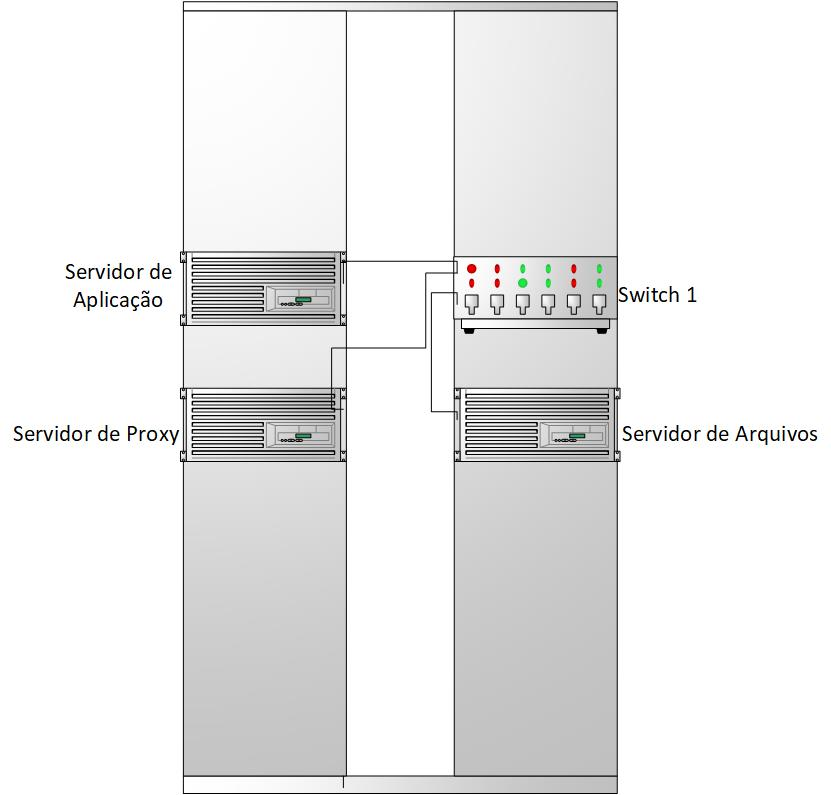
\includegraphics[scale=0.4]{rack1}        \\ \hline
2        & Rack 2        & 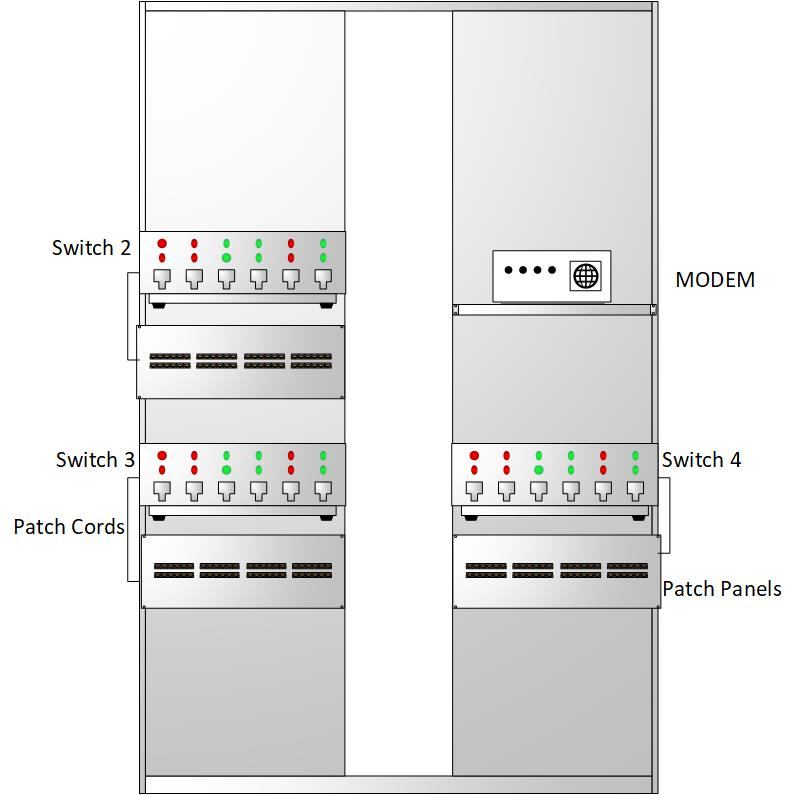
\includegraphics[scale=0.4]{rack2}        \\ \hline
\end{tabular}
\end{table}